% ===== RUBRIC OF TEACHER'S JOB ASPECTS =====

% A single rubric criterion
\newcommand{\rubriccriterion}[4]{
\stepcounter{rubricquestion}
\section*{\therubricquestion: #1}

\smallskip
\note{Unaware:} #2

\note{Beginner:} #3

\note{Guru:} #4

\medskip
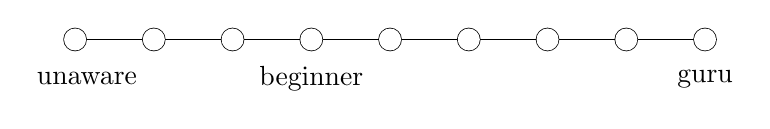
\begin{tikzpicture}
\draw (0,0) -- (8,0);
\foreach \i in {0,1,...,8} % numbers on line
{
\fill[black] (\i,0) circle (1.5 mm);
\fill[white] (\i,0) circle (1.4 mm);
}
\node at (0.15, -0.5) {unaware};
\node at (3, -0.5)    {beginner};
\node at (8, -0.5)    {guru};
\end{tikzpicture}
}

\restoregeometry
\chapter*{Rubric for teaching skills}
\label{rubric}

The following pages present a scoring rubric for teaching skills. Many teachers (young and old alike) don't perceive all the different levels and dimensions of the teaching skill. This is often caused by them not seeing these skills on others. After months or years teaching, there may come a moment when you realize that the space for improvement is much bigger that you initially expected.\punct{.}\footnote{More information can be found for example in the book \emph{How Learning Works: Seven Research-Based Principles for Smart Teaching}.}

\section*{Waht is a scoring rubric?}

The scoring rubric is a self-assessment tool (helping you see and describe your own skills and knowledge).
It helps you to perceive and name all the fundamental parts of a concept (e.g.\ being able to program means being able t design an angorithm, work with memoty effectively, know the syntax, \dots) and evaluate your competence in these parts (e.g.\ I'm able to design an effective algorithm, though it's a bit problematic for me to express it in code and I don't optimize memory usage at all).

\section*{How to use the rubric for teaching skills?}

Fill in the rubric at the beginning of the semester (indicate the level of your skill on the scale). Choose 1--3 areas you want to focus on this semester. If you want to be thorough, try to think of specific actions to do and useful indicators of your progress. Go over the rubric again at the end of the semester and reevaluate your progress in individual areas.

Another option is to treat the rubric as a manifesto -- the \enquote{guru} descriptions represent our view of the skills great teachers have. These we would like to cultivate within the starting teachers as well.

\newcounter{rubricquestion}

\newpage
\rubriccriterion{Conscious attention, following goals, tracking}
{My lectures don't have a clearly set goal. When teaching, I'm unaware of the current situation or direction. I often feel lost.}
{Sometimes I see my current goal and understand effects of the methods I'm using at that moment. Most of the time, however, I'm not consciously paying attention to my teaching.}
{I'm almost always paying attention to what happens to me and the class, what I'm doing, what effects it'll have and what goals I follow. I know how we arrived to the current situation.}

\rule{\textwidth}{0.4pt}
\rubriccriterion{Class interaction, asking public questions}
{I don't interact with the class. I don't ask since I would probably not get answers. I don't know how to engage students.}
{I know it's possible to interact with the class and I know the tools to do it. Nevertheless, I'm unable to use them well. Sometimes when I ask, I don't get answers.}
{I interact with the class often and do it in a way that engages the students. I can effortlessly solve the situations when I'm not getting answers (e.g.\ by question reformulation).}

\newpage
\rubriccriterion{Strukturování výuky}
{O strukturování výuky nijak nepřemýšlím.}
{Chápu smysl přehledného strukturování své hodiny a snažím se o to. Často se ale zamotám, ztratím nit, nebo řeším mnoho naráz a studenti se pak ztrácí nebo odpojují.}
{Moje hodiny mají jasnou strukturu. Studenti ví, co se právě děje, co bude následovat a chápou návaznosti. Mezi jednotlivými bloky vědomě dělám zřetelné přechody.}

\rule{\textwidth}{0.4pt}
\rubriccriterion{Vlastní pocit z výuky}
{Svou výuku nijak nereflektuji.}
{Ve výuce si často moc nevěřím, vyžaduje to hodně energie, nebo se cítím napjatě. Mám strach z toho, na co se studenti zeptají.}
{Ve výuce se většinou cítím uvolněně a sebevědomě, mám svůj styl a baví mě to.}

\newpage
\rubriccriterion{Formativní zpětná vazba}
{O dávání zpětné vazby studentům nijak nepřemýšlím.}
{Snažím se studentům zpětnou vazbu dávat. Myslím si však, že jí není dost, nebo to nedělám efektivně, nebo to studenti nevnímají jako podporu a projev respektu.}
{Se studenty ve výuce interaguji tak, že dostávají průběžně formativní zpětnou vazbu. Chápou tedy, co jim jde, kde dělají chyby a jak se mohou zlepšovat. Zároveň se moji studenti cítí být respektováni a zpětné vazby se nebojí.}

\rule{\textwidth}{0.4pt}
\rubriccriterion{Jasné zadávání úloh}
{O zadávání úloh nijak zvlášť nepřemýšlím.}
{Stává se mi, že zadám úlohu a studenti neví, co dělat, jak začít nebo k čemu mají dojít (co má být výsledkem).}
{Když zadávám úlohu nebo aktivitu, mají studenti jasno v tom, co mají dělat a neřeší tak zbytečně věci, které nemám záměr procvičovat.}

\newpage
\rubriccriterion{Design výuky a variabilita aktivit}
{Učím tak, jak mi řekli nebo kopíruji výuku, kterou jsem viděl(a). Nepřemýšlím o~jiných variantách.}
{Jsem si vědom(a) toho, že existuje mnoho typů aktivit, které lze při výuce použít. Neznám jich ale dostatek, nedokážu je efektivně zadávat, nebo nemám jasno v tom, proč je vybírat.}
{Znám dostatek typů aktivit, svou výuku skládám tak, aby byla dostatečně pestrá. Vybrané aktivity efektivně učí/procvičují to, co mám záměr učit/procvičovat. Vybrané aktivity zároveň studenty efektivně zapojují a přispívají k jejich motivaci.\vspace{-0.5em}}

\rule{\textwidth}{0.4pt}
\rubriccriterion{Širší kontext výuky a konkrétní hodiny}
{O širším kontextu výuky nepřemýšlím.}
{Uvědomuji si, že nemám pro sebe pojmenované znalosti a dovednosti, které u~studentů rozvíjím. Nevím, jak jejich pokrok sledovat. Nevím, v jakém kontextu to studenti využijí.}
{Mám jasnou představu o tom, k čemu studenty vedu, jaké dovednosti rozvíjím, jaké znalosti jim chci předat. Vím, proč tyto dovednosti rozvíjím a v jakém kontextu je studenti v budoucnu použijí. Vím, jak jejich pokrok sledovat.}
\vspace*{-1em}

\newpage
\rubriccriterion{Jasné vysvětlování}
{Svoje vysvětlování nijak nereflektuji.}
{Když vysvětluji, běžně se mi stává, že si nejsem jistý, zda vysvětluji dobře a zda to studentům pomáhá při pochopení.}
{Když vysvětluji teorii, demonstruji řešení nebo opravuji chybný postup. Dělám to efektivně a dokážu se dobře vžít do toho, jak to vidí student. Nestává se mi, že by studenti moje vysvětlení nechápali, nebo že bych vysvětloval(a) něco, na co se neptali.}

\rule{\textwidth}{0.4pt}
\rubriccriterion{Nastavení prostředí, systémy ve výuce}
{O nastavení atmosféry nepřemýšlím, systémy ve své výuce nevnímám.}
{Přemýšlím o nastavení pravidel i atmosféry. Systémy ve výuce (např. bodování) přebírám od ostatních. Nemám ale jasno v efektech, nebo neznám způsoby, jak je lze upravit.}
{Umím ve výuce vytvořit prostředí, které podporuje efektivní učení. U systémů, které používám (např. bodování, bonbóny, zahajovací rituály) chápu efekt. Systémy nepřebírám slepě, chápu jejich účel a uzpůsobuji podle svých potřeb.}

\newpage
\rubriccriterion{Improvizace, přizpůsobování}
{V průběhu své výuky na vzniklé situace nijak vědomě nereaguji.}
{Uvědomuji si chvíle, kdy by mohlo být zajímavé nebo užitečné dělat něco jiného, než jsem měl(a) v plánu. Většinou ale nedokážu v daný moment vhodně zareagovat.}
{Dokážu svoji výuku průběžně přizpůsobovat tomu, co se právě děje ve skupině a co studenti potřebují. Mám k tomu dostatek nástrojů a dokážu je efektivně použít.}

\rule{\textwidth}{0.4pt}
\rubriccriterion{Individuální interakce se studenty}
{O konzultacích nijak vědomě nepřemýšlím.}
{Stává se mi, že si nevím rady při individuální interakci se studentem (např. u~tabule, konzultace). Interakce neprobíhá efektivně nebo se student cítí zastrašen.}
{Při interakcích s jednotlivci (např. u tabule, konzultace) efektivně využívám čas. Studenti se mnou konzultují rádi, cítí ze mě respekt a podporu.}

\newpage
\rubriccriterion{Management skupiny, \textit{subgrouping}}
{Přijde mi, že dělit skupinu je zbytečnost, o~práci v~menších skupinkách nepřemýšlím.}
{Uvědomuji si možnosti práce ve dvojicích či menších skupinách. Tuším, že bych toho mohl(a) lépe využívat, hledám jak.}
{Mám jasno v tom, kdy chci pracovat se skupinou jako celkem, kdy s jednotlivci a kdy se skupinkami. Rozdělení do menších skupin efektivně používám. Ve vhodných případech zadávám interakce mezi skupinami.}

\rule{\textwidth}{0.4pt}
\rubriccriterion{Čtení skupiny}
{Skupinu ve své výuce nesleduji, pozornost věnuji pouze obsahu.}
{Uvědomuji si, že mi skupina vysílá signály a že by bylo dobré jim rozumět a využít je pro efektivní vedení výuky. Ve výuce to ale dokážu jen výjimečně.}
{Dokážu dobře odhadnout naladění skupiny. Mám jasno v tom, co se ve skupině studentů děje (např. únava, rezignace, zájem).}
